\documentclass[a4,center,fleqn]{NAR}


\usepackage{NAR-natbib}
\bibliographystyle{unsrtnat}
\usepackage{color}
\newcommand{\rngcomment}[1]{{\color{red}RNG: #1}}
\newcommand{\bkmcomment}[1]{{\color{blue}BKM: #1}}
% Enter dates of publication
\copyrightyear{2008}
\pubdate{31 July 2009}
\pubyear{2009}
\jvolume{37}
\jissue{12}

\articlesubtype{Genomics and Bioinformatics}

\begin{document}

\title{Article title}

\author{%
Brian K. Mannakee\,$^{1}$ and
Ryan N. Gutenkunst\,$^{2}$%
\footnote{To whom correspondence should be addressed.
Email: rgutenk@email.arizona.edu}}

\address{%
$^{1}$University of Arizona Mel and Enid Zuckerman College of Public Health
and
$^{2}$University of Arizona Department of Molecular and Cellular Biology}
% Affiliation must include:
% Department name, institution name, full road and district address,
% state, Zip or postal code, country

\history{%
Received January 1, 2009;
Revised February 1, 2009;
Accepted March 1, 2009}

\maketitle

\begin{abstract}
Text. Text. Text. Text. Text. Text. Text. Text. Text. Text. Text.
Text. Text. Text. Text. Text. Text. Text. Text. Text. Text. Text.
Text. Text. Text. Text. Text. Text. Text. Text. Text. Text. Text.
Text. Text. Text. Text. Text. Text. Text. Text. Text. Text. Text.
Text. Text. Text. Text. Text. Text. Text. Text. Text. Text. Text.
Text. Text. Text. Text. Text. Text. Text. Text. Text. Text. Text.
Text. Text. Text. Text. Text. Text. Text. Text. Text. Text. Text.
Text. Text. Text. Text. Text. Text. Text. Text. Text. Text. Text.
Text. Text.
\end{abstract}


\section{Introduction}

Cancer develops as the result of the accumulation of somatic mutations and clonal selection of cells with mutations that confer a selective advantage on the cell.
Understanding the forces that shaped the evolutionary history of a tumor, the mutations that are responsible for its growth, the rate at which mutations are occurring, or how much genetic diversity is likely present in the tumor, requires accurate variant calling, particularly at low variant allele frequency \cite{Williams2016,Bozic2016,Williams2018}.
Accurate variant identification is also critical in optimizing the treatment regime for an individual patients disease \citep{Ding2012,Mardis2012,Chen2013,Borad2014,Findlay2016}.
Low frequency mutations present a significant problem for current mutation calling methods because their signature in the data is difficult to distinguish from the noise introduced by Next Generation Sequencing (NGS), and this problem increases as sequencing depth increases.

Methods for identifying true somatic mutations - i.e. variant calling -  from NGS data are an active area of research in bioinformatics.
The earliest widely used somatic variant callers aimed specifically at tumors, Mutect1 and Varscan2, used a combination of heuristic filtering and a model of sequencing errors to identify and score potential variants, setting a threshold for that score designed to balance sensitivity and specificity \citep{Koboldt2012,Cibulskis2013}.
Subsequent research gave rise to a number of alternate variant calling strategies including haplotype based callers \citep{Garrison2012},
joint genotype analysis (SomaticSniper, JointSNVMix2, Seurat, and CaVEMan,MuClone)\citep{Larson2012,Roth2012a,Christoforides2013,Jones2016,Dorri2019}, allele frequency based analysis (Strelka, MuTect, LoFreq, EBCall, deepSNV, LoLoPicker, and MuSE)\citep{Saunders2012,Wilm2012,Shiraishi2013b,Gerstung2012,Carrot-Zhang2017,Fan2016}, and a mixture of ensemble and deep learning methods (MutationSeq, SomaticSeq, SNooPer, and BAYSIC).
All of these methods have varying levels of complexity, and some are focused on specific types of data.
The one thing they all have in common is that they either implicitly or explicitly assume that the probability of a mutation occuring at a particular site is proportional to the overall mutation rate, and the same at every site in the genome.

Single nucleotide substitions, i.e. simple mutations, arise in tumors at a rate and at genomic locations driven by two main processes. 
The first is the spontaneous accumulation of mutations that occurs in all dividing tissues, and has a characteristic mutation signature that describes the probability of mutation in a given genomic context \citep{Nik-Zainal2012a,Alexandrov2015,Lee-Six2018}. 
The second, and far more complex, process is the accumulation of mutations through exposure to mutagens or degradation - via mutation or deletion - of cellular machinery responsible for the identification and repair of damage or replication errors. 
Many mutagens and DNA repair mechanism defects also have highly specific mutation signatures, such that they can be identified by observing the mutations in the tumor \citep{Alexandrov2013a,Helleday2014a,Nik-Zainal2016,Kandoth2013,Alexandrov2016}.

Here we present an algorithm for estimating the prior probability of mutation at a given site using the observed mutation spectrum of the tumor as well as its mutation rate, and show that the addition of this prior to the MuTect variant calling model produces a superior variant classifier in both simulated and real tumor data.
We then extend the method with an application of the local false discovery rate by computing the probability that a site is non-null under an assumption of clonal expansion with either early or small selective differences between clones.
We provide a simple implementation in R that takes MuTect caller output as input, and returns the posterior probability that a site is variant for every site observed by MuTect.



\section{MATERIALS AND METHODS}

\subsection{Base probability model}

At every site in the genome with non-zero coverage, Next Generation Sequencing (NGS) produces a vector $\mathbf{x}  = (\{b_i\},\{q_i\}), i = 1\dots D$ of base calls and their associated quality scores, where $D$ is total read depth.
The goal is to use $\mathbf{x}$ to select between competing hypotheses;
\begin{equation*}
\begin{array}{l}
\mathbf{H_0}:\quad \textrm{Alt allele} = m;\quad\nu = 0\\
\mathbf{H_1}:\quad \textrm{Alt allele} = m;\quad\nu = \hat{f},
\end{array}
\end{equation*}

where $\nu$ is the variant allele frequency, $\hat{f}$ is the maximum likelihood estimate of $\nu$ given data $\mathbf{x}$, i.e. the ratio of the count of variant reads and total read depth, and $m$ is any of the 3 possible alternative non-reference bases.
For a given read with base $b_i$ and q-score $q_i$, the density function under a particular hypothesis is defined as

\begin{equation*}
  \textrm{f}_{\nu,m}(b_i,q_i) = \left\{
    \begin{array}{cr}
      \nu \frac{10^{-q_i/10}}{3} + (1-\nu)(1-10^{-q_i/10}) & b_i = \textrm{reference}\\
      \nu(1-10^{-q_i/10}) + (1-\nu) \frac{10^{-q_i/10}}{3} & b_i = m\\
      \frac{10^{-q_i/10}}{3} & otherwise.
    \end{array}
    \right.
\end{equation*}

The likelihood under the hypothesis is then $\mathcal{L}_{\nu,m}(\mathbf{x}) = \prod_{i=1}^{D} \textrm{f}_{\nu,m}(x_i)$.
MuTect reports the log likelihood ratio $\mathrm{log}(\mathcal{L}_{\nu=\hat{f},m}(\mathbf{x})/\mathcal{L}_{\nu=0,m}(\mathbf{x}))$ as either TLOD or \textrm{t\_lod\_fstar} depending on the version.
By fixing the threshold posterior odds at two, the site-specific mutation probability a constant $\mathrm{p}(M)= \mu = 3\mathrm{e}{-6}$, and $\mathrm{p}(m \mid M)$ the prior probability of mutation to specific allele $m$ constant $\mathrm{p}(m \mid M) = \mu/3 = 1\mathrm{e}{-6}$, they derive a TLOD threshold of 6.3 for classifying a site as a somatic variant.



\subsection{Estimation of the mutation signature.}

While variant calling algorithms typically assume a constant probability of mutation at every site in the genome, work by Alexandrov and others show that the random mutation generating process actually varies from site to site in a nucleotide context specific manner.
We develop a model of the prior probability of mutation to allele $m$ conditional on the observed genomic context $\mathrm{p}(m,M \mid C)$, and demonstrate an empirical Bayes method for computing this probability from MuTect output.
The prior probability $\mathrm{p}(m,M \mid C)$ can be decomposed as
$$
\mathrm{p}(m,M \mid C) = \mathrm{p}(m \mid C) \mathrm{p}(M \mid C) = \mathrm{p}(m \mid C) \mathrm{p}(C \mid M)\frac{p(M)}{p(C)}
$$
since the probability of a mutation at a site and the probability that it is to allele $m$ are independent conditional on the context.
Here $\mathrm{p}(M) = \mu$ as above, and the empirical distribution of contexts $\mathrm{p}(C)$ is the fraction of the genome made up of each context.
We model $\mathrm{p}(C \mid M)$ as a multinomial distribution with parameter $\boldsymbol{\pi} = \{\pi_i\}, i = 1\dots96$.
Mutations are drawn from this multinomial distribution such that $\mathrm{p}(C = i \mid M) = \pi_i$.
The final quantity $\mathrm{p}(m \mid C)$, the probability of mutation to $m$ given a particular three letter context, is a function of $\boldsymbol{\pi}$. 
We are left to estimate only the vector of probabilities $\boldsymbol{\pi}$.


$$
\begin{aligned}
C \mid M,\boldsymbol{\pi} & \sim \textrm{Multinomial}(\boldsymbol{\pi})  \\
\boldsymbol{\pi} \mid \boldsymbol{\alpha} &\sim \textrm{Dirichlet}(\boldsymbol{\alpha}).
\end{aligned}
$$

The posterior distribution of $\boldsymbol{\pi}$ is $\boldsymbol{\pi} \mid C,\boldsymbol{\alpha} \sim \textrm{Dirichlet}(\mathbf{C} + \boldsymbol{\alpha})$, where $\mathbf{C} = (C_1,\dots,C_{96})$ are the counts of mutations present in the tumor for each of the 96 contexts.
We compute an empirical bayes estimate of $\boldsymbol{\pi}$ by choosing $\mathbf{C}$ as the set of mutations assigned a TLOD by MuTect above some threshold, which we choose as 10.
We show through extensive simulation that our estimate of $\boldsymbol{\pi}$ converges quickly its true simulated value.

Returning to the model above, we can calculate the log posterior odds in favor of $\mathbf{H_1}$ as

$$
  \textrm{log}_{10} \left(\frac{(\mathcal{L}_{\nu=\hat{f},m}(\mathbf{x})\mathrm{p}(m,M \mid C)}{(\mathcal{L}_{\nu=0,m}(\mathbf{x})(1-\mathrm{p}(m,M \mid C))} \right) = \textrm{TLOD} + \textrm{log prior odds},
$$

and the posterior odds ratio in favor of $\mathbf{H_1}$ as
$$
10^{(\textrm{TLOD} + \textrm{log prior odds})}.
$$

We show via extensive simulation that under the assumption that the mutation signature describes the biological process generating mutations in a tumor, our posterior odds ratio is a better classifier than MuTect at any threshold.
Unfortunately, this increased classification performance comes at a cost in terms of calibration, The probabilities from this model are substantially worse than those from Mutect, such that threshold selection is essentially impossible and precision/recall is substantially worse for this model.
There are several distributional assumptions in this model that effect model calibration, and we address all of them below.

\subsection{Estimation of the mutation rate.}

As discussed above, MuTect fixes the site-specific mutation probability at $\mathrm{p}(M)= \mu = 3\mathrm{e}{-6}$.
All variant callers we are aware of either fix this parameter $\mu$ or allow the user to input the value, but there is no way to really know this value until the variant allele frequencies have been observed.
As with estimation of the mutation signature, we can use high confidence mutations and a model of tumor evolution to compute the tumor-specific mutation rate.
\citet{Bozic2016} show that for any variant allele frequency $\alpha$, the total number of mutations with frequency greater than $\alpha$ and less than $0.25$ is

$$
N(\alpha) = N\mu \left( \frac{1}{\alpha} - \frac{1}{0.25} \right)
$$

Where $N$ is the total number of sites sequenced and $\mu$ is the per-site mutation probability.
By selecting $\alpha$ such that we are highly confident in all calls at frequencies greater than $\alpha$, we can compute $\mu$ and recompute the odds in favor of $\mathbf{H_1}$.


%`\subsection{False positive rate control.}

%We develop a method, following \citet{Efron2008}, for controlling the false positive rate.
%Every site with sufficient coverage and at least 1 alternate read falls into one of two classes, they are either \textit{null} (non-variant with $\nu = 0$) or \textit{nonnull} (variant with $\nu = \hat{f}$) with prior probabilities $p_0$ and $p_1 = 1-p_0$,

%$$
%\begin{array}{ll}
%p_0 = \textrm{P}\{\textrm{null}\} \quad & \textrm{f}_{0}(\mathbf{x}) \quad \textrm{density if null}\\
%p_1 = \textrm{P}\{\textrm{nonnull}\} \quad & \textrm{f}_{1}(\mathbf{x}) \quad \textrm{density if nonnull} .
%\end{array}
%$$

%The local, or site-specific, true positive probability $p_1$ can be estimated as the fraction of all sequenced sites that are expected to be positive.
%In a neutrally evolving tumor, the number of cells is growing exponentially, and the count of variants with an allele frequency greater than a given allele frequency $f$ is \cite{Bozic2016,Williams2016a}.
%$$
%N(f) = \frac{N\mu}{f},
%$$
%Where $N$ is the total number of sites sequenced and $\mu$ is the per-site mutation probability.
%The estimated fraction of all of the sites in the genome that will have a mutation with frequency $f$ is
%$$
%\hat{p}_1 = \frac{\int_{f_{-}}^{f_{+}} N(f)}{N} = \frac{\mu}{f - .01} -  \frac{\mu}{f + .01}
%$$

%\bkmcomment{This is wrong. This is the cdf. I need the integral of the derivative which is the density.}
%and the estimated null probability $\hat{p}_0 = 1 - \hat{p}_1$.
%\citet{Williams2016a} provides a full derivation for this, we are essentially computing the integral here of $N(f)$ in a small area around $f$.


\subsection{Tumor simulations.}

We simulated realistic variant sites and allele frequencies using a branching process to simulate neutral evolution with no death.
Variants were selected from TCGA and PCAWG variant files(dates).
Whole genome (100X depth), and whole exome (500X depth) reads from the GRCH38 reference genome with VarSim \cite{Mu2015}, and aligned them to GRch38 with BWA \cite{Li2009a}, both with default parameters.
Variants were spiked to create tumors with Bamsurgeon with default parameters \cite{Ewing2015a},
and called with MuTect 1.1.7 \cite{Cibulskis2013} with the following parameters:

\begin{tiny}
\begin{verbatim}

  java -Xmx24g -jar $MUTECT_JAR --analysis_type MuTect --reference_sequence $ref_path \
        --dbsnp $db_snp \
        --enable_extended_output \
        --fraction_contamination 0.00 \
        --tumor_f_pretest 0.00 \
        --initial_tumor_lod -10.00 \
        --required_maximum_alt_allele_mapping_quality_score 1 \
        --input_file:normal $tmp_normal \
        --input_file:tumor $tmp_tumor \
        --out $out_path/$chr.txt \
        --coverage_file $out_path/$chr.cov

\end{verbatim}
\end{tiny}
Variants identified by MuTect are labelled as to whether they pass all MuTect filters, pass all filters *other* than the evidence threshold \textrm{tlod\_f\_star}, or fail to pass any filter other than \textrm{tlod\_f\_star}. Variants that pass all filters or fail only \textrm{tlod\_f\_star} are then passed to {method} for prior estimation and rescoring.

\subsection{Real tumor data.}
\subsubsection{Acute Myeloid Leukemia}
We downloaded the whole genome sequence for aml31 \bkmcomment{citation and download date}.
We merged the gold and platinum lists, and define is \textit{not present} any variant for which deep sequencing was performed and zero alternate reads were observed.
This is a very conservative metric.


\begin{figure}[t]
\begin{center}
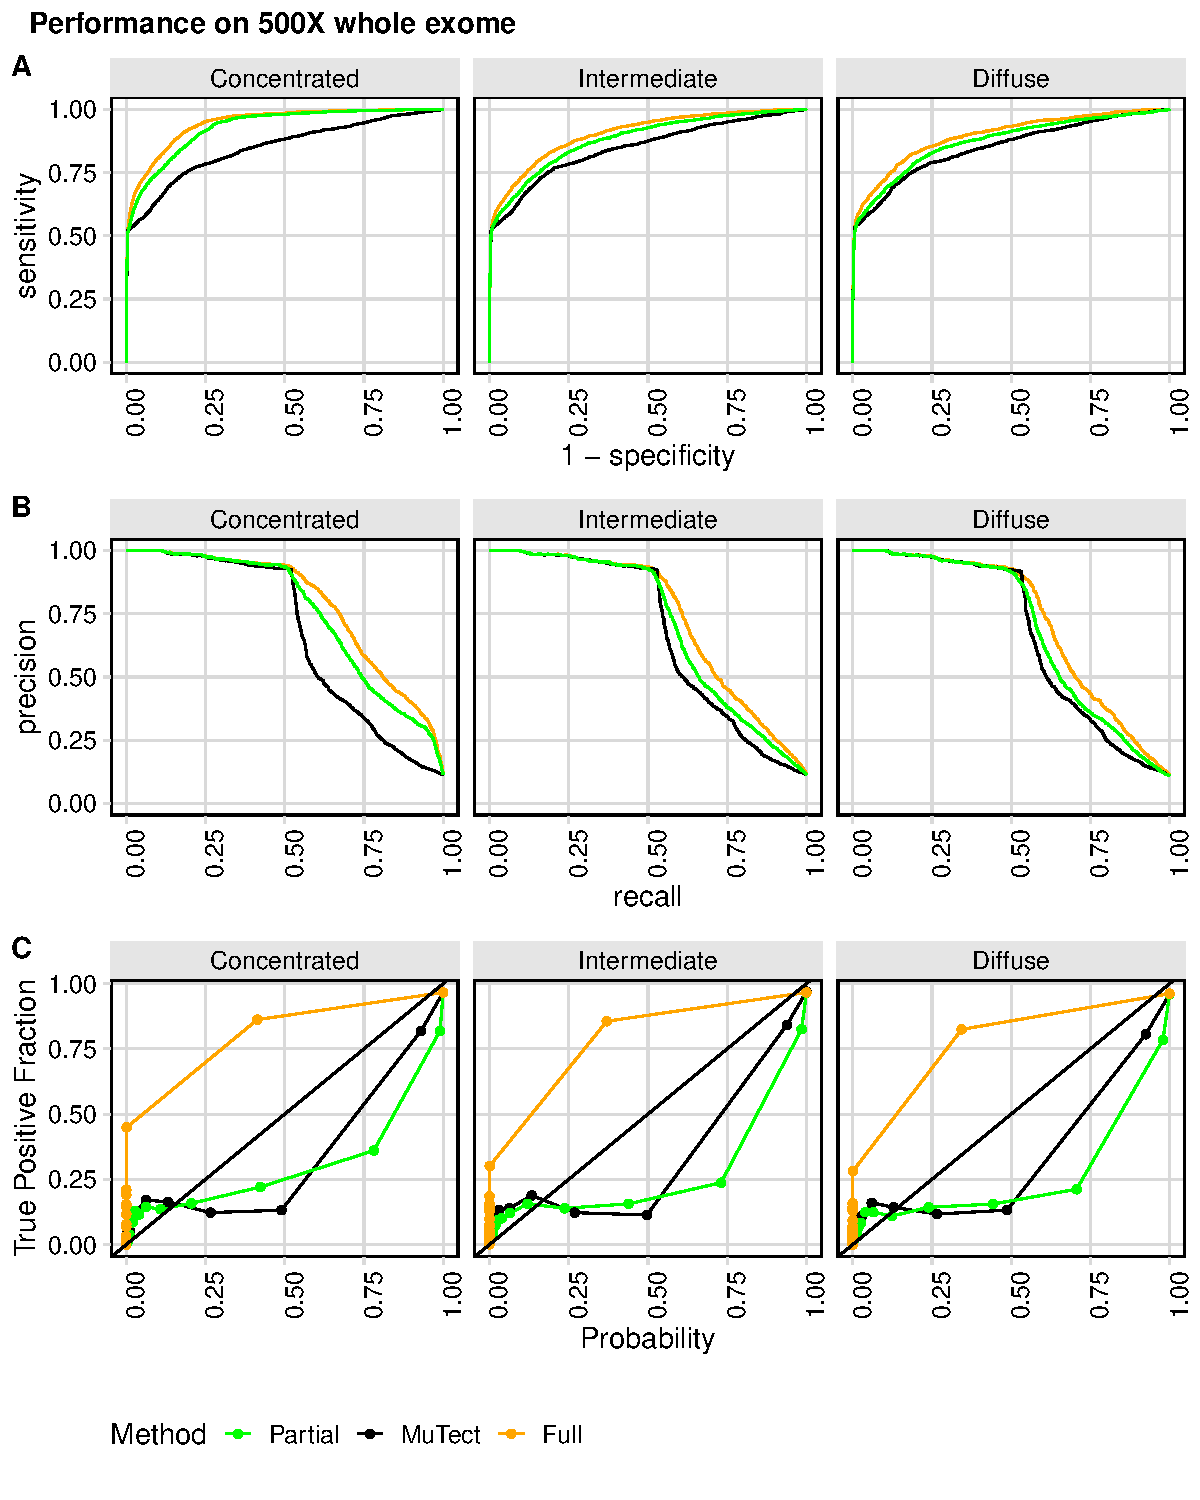
\includegraphics{figures/wes_left_plot.pdf}
\end{center}
\caption{Caption for figure within column.}
\label{NAR-fig1}
\end{figure}


\section{RESULTS}

\subsection{Results subsection one}

Text. Text. Text. Text. Text. Text. Text. Text. Text. Text. Text.
Text. Text. Text. Text. Text. Text. Text. Text. Text. Text. Text.
Text. Text. Text. Text. Text. Text. Text. Text. Text. Text. Text.
Text. Text. Text. Text. Text. Text. Text. Text. Text. Text. Text.
Text. Text. Text. Text. Text. Text. Text. Text. Text. Text. Text.
Text. Text. Text. Text. Text. Text. Text. Text. Text. Text. Text.
Text. Text. Text. Text. Text. Text. Text. Text. Text. Text. Text.
Text. Text. Text. Text. Text. Text. Text. Text. Text. Text. Text.
Text. Text. Text. Text. Text. Text. Text. Text. Text. Text. Text.
Text. Text. Text. Text. Text. Text. Text. Text. Text. Text. Text.
Text. Text. Text. Text. Text. Text. Text. Text. Text. Text. Text.
Text. Text. Text. Text. Text. Text. Text. Text. Text.

\begin{table}[b]
\tableparts{%
\caption{This is a table caption}
\label{table:01}%
}{%
\begin{tabular*}{\columnwidth}{@{}lllll@{}}
\toprule
Col. head 1 & Col. head 2 & Col. head 3 & Col. head 4 & Col. head 5
\\
& (\%) & (s$^{-1}$) & (\%) & (s$^{-1}$)
\\
\colrule
Row 1 & Row 1 & Row 1 & -- & --
\\
Row 2 & Row 2 & Row 2 & Row 2 & Row 2
\\
\botrule
\end{tabular*}%
}
{This is a table footnote}
\end{table}


\subsection{Results subsection two}

Text.  Text. Text. Text. Text. Text. Text. Text. Text. Text. Text.
Text. Text. Text. Text. Text. Text. Text. Text. Text. Text. Text.
Text (see Table \ref{table:01}).

Text. Text. Text. Text. Text. Text.
Text. Text. Text. Text. Text. Text. Text. Text. Text. Text. Text.
Text. Text. Text. Text. Text. Text. Text. Text. Text.
Text (see Figure \ref{NAR-fig2}a).

Text. Text. Text. Text. Text.
Text. Text. Text. Text. Text. Text. Text. Text. Text. Text. Text.
Text. Text. Text. Text. Text. Text. Text. Text. Text. Text. Text.
Text. Text. Text. Text. Text. Text. Text. Text. Text. Text. Text.
Text. Text. Text. Text. Text. Text. Text. Text. Text. Text. Text.
Text. Text. Text. Text. Text. Text. Text. Text. Text. Text. Text.
Text. Text. Text. Text. Text. Text. Text. Text. Text. Text. Text.
Text. Text. Text. Text. Text. Text. Text. Text. Text. Text. Text.
Text. Text. Text. Text. Text. Text. Text. Text. Text. Text. Text.
Text. Text. Text. Text. Text. Text. Text. Text. Text. Text. Text.
Text. Text. Text. Text. Text. Text. Text. Text. Text. Text. Text.
Text. Text. Text. Text. Text. Text. Text. Text. Text. Text.

\begin{figure*}[t]
\begin{center}
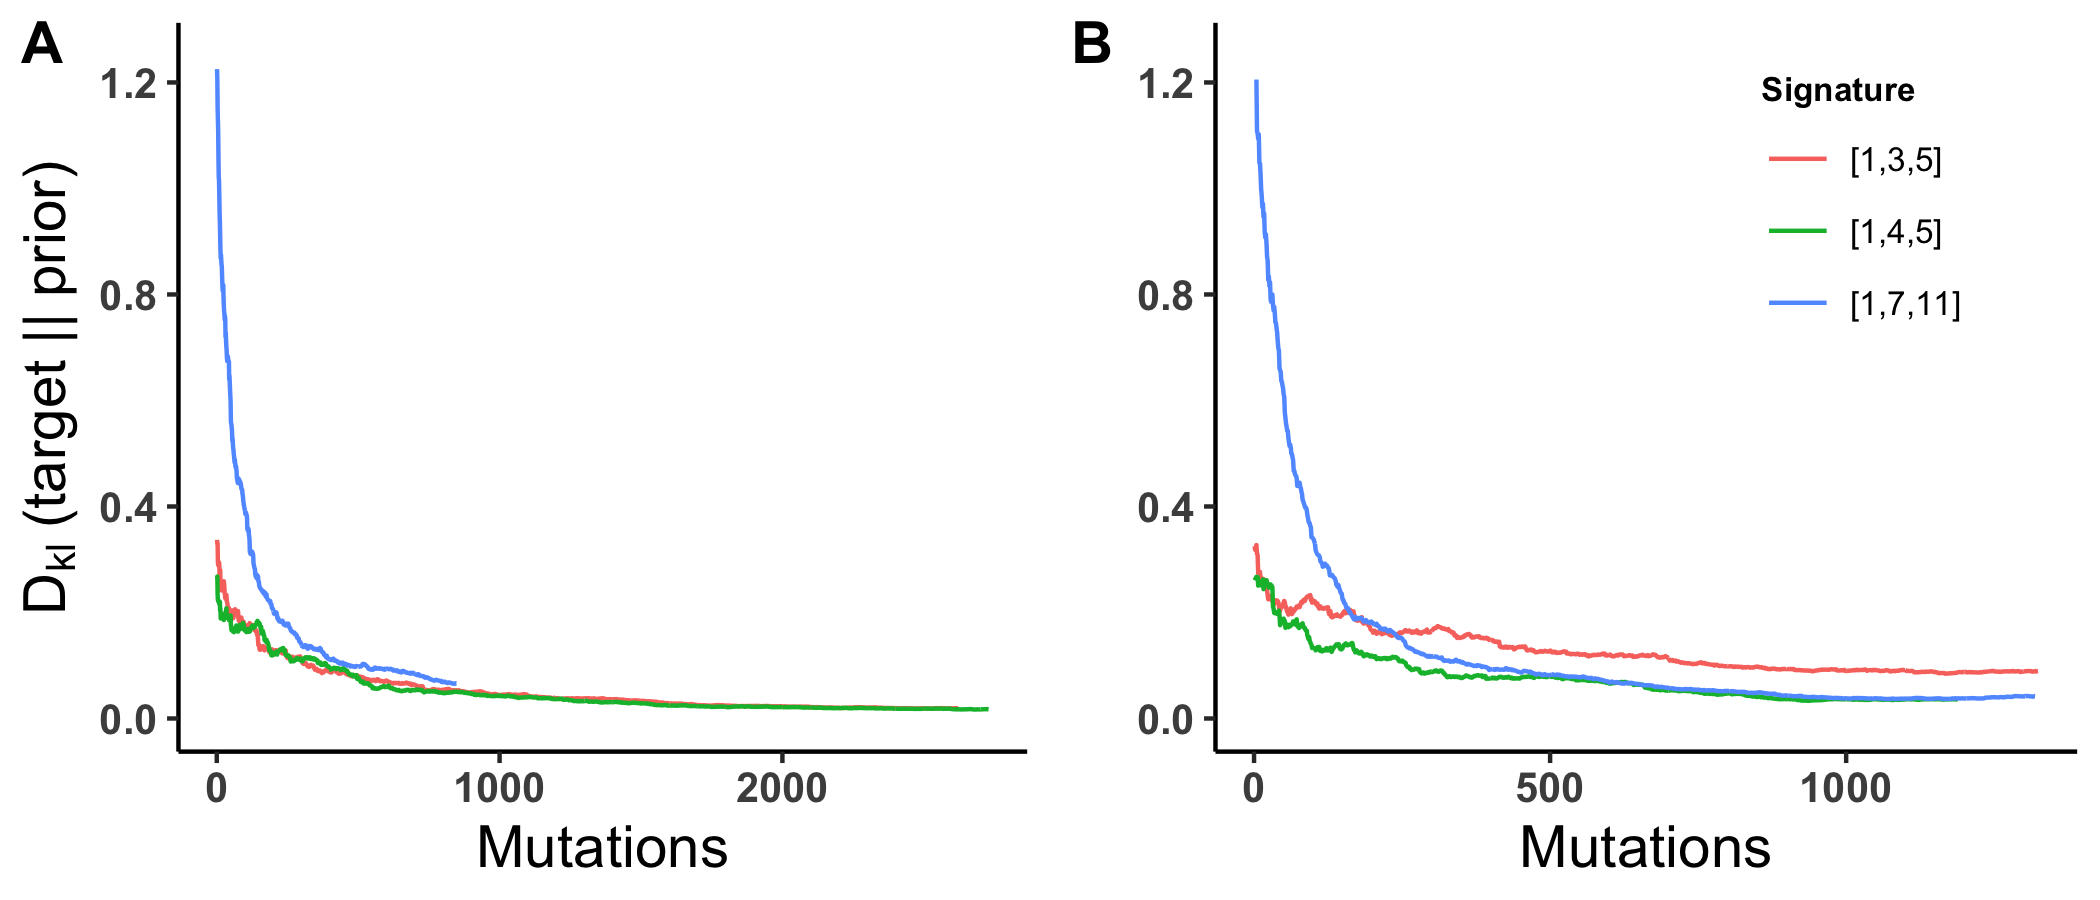
\includegraphics{figures/kl_figure.png}
\end{center}
\caption{Caption for wide figure over two columns.
\textbf{(a)} Left figure.
\textbf{(b)} Right figure (see (a)).
}
\label{NAR-fig2}
\end{figure*}


\subsection{Results subsection three}

Text. Text. Text. Text. Text. Text. Text. Text. Text. Text. Text.
Text. Text. Text. Text. Text. Text. Text. Text. Text. Text. Text.
Text. Text. Text. Text. Text. Text. Text. Text. Text. Text. Text.
Text. Text. Text. Text. Text. Text. Text. Text. Text. Text. Text.
Text. Text. Text. Text. Text. Text. Text. Text. Text. Text. Text.
Text. Text. Text. Text. Text. Text. Text. Text. Text. Text. Text.
Text. Text. Text. Text. Text. Text. Text. Text. Text. Text. Text.
Text. Text. Text. Text. Text. Text. Text. Text. Text. Text. Text.
Text. Text. Text. Text. Text. Text. Text. Text. Text. Text. Text.
Text. Text. Text. Text. Text. Text. Text. Text. Text. Text. Text.
Text. Text. Text.


\section{DISCUSSION}

\subsection{Discussion subsection one}

Text. Text. Text. Text. Text. Text. Text. Text. Text. Text. Text.
Text. Text. Text. Text. Text. Text. Text. Text. Text. Text. Text.
Text. Text. Text. Text. Text. Text. Text. Text. Text. Text. Text.
Text. Text. Text. Text. Text. Text. Text. Text. Text. Text. Text.
Text. Text. Text. Text. Text. Text. Text. Text. Text. Text. Text.
Text. Text. Text. Text. Text. Text. Text. Text. Text. Text. Text.
Text. Text. Text. Text. Text. Text. Text. Text. Text. Text. Text.
Text. Text. Text. Text. Text. Text. Text. Text. Text. Text. Text.
Text. Text. Text. Text. Text. Text. Text. Text. Text. Text. Text.
Text. Text. Text. Text. Text. Text. Text. Text. Text. Text. Text.
Text. Text. Text. Text. Text. Text. Text. Text. Text. Text. Text.
Text. Text. Text. Text. Text. Text. Text. Text. Text. Text. Text.
Text. Text. Text. Text. Text. Text. Text. Text. Text. Text. Text.
Text. Text. Text. Text. Text. Text. Text. Text. Text. Text. Text.
Text. Text. Text. Text. Text. Text. Text. Text. Text. Text. Text.
Text. Text. Text. Text. Text. Text. Text. Text. Text. Text. Text.
Text. Text. Text. Text. Text. Text. Text. Text. Text. Text. Text.
Text. Text. Text. Text. Text. Text. Text. Text. Text. Text. Text.
Text. Text. Text. Text. Text. Text. Text. Text. Text. Text. Text.
Text. Text. Text. Text. Text. Text. Text. Text. Text. Text. Text.
Text. Text. Text. Text. Text. Text.


\subsection{Discussion subsection two}

Text. Text. Text. Text. Text. Text. Text. Text. Text. Text. Text.
Text. Text. Text. Text. Text. Text. Text. Text. Text. Text. Text.
Text. Text. Text. Text. Text. Text. Text. Text. Text. Text. Text.
Text. Text. Text. Text. Text. Text. Text. Text. Text. Text. Text.
Text. Text. Text. Text. Text. Text. Text. Text. Text. Text. Text.
Text. Text. Text. Text. Text. Text. Text. Text. Text. Text. Text.
Text. Text. Text. Text. Text. Text. Text. Text. Text. Text. Text.
Text. Text. Text. Text. Text. Text. Text. Text. Text. Text. Text.
Text. Text. Text. Text. Text. Text. Text. Text. Text. Text. Text.
Text. Text. Text. Text. Text. Text. Text. Text. Text. Text. Text.
Text.

Text. Text. Text. Text. Text. Text. Text. Text. Text. Text. Text.
Text. Text. Text. Text. Text. Text. Text. Text. Text. Text. Text.
Text. Text. Text. Text. Text. Text. Text. Text. Text. Text. Text.
Text. Text. Text. Text. Text. Text. Text. Text. Text. Text. Text.
Text. Text. Text. Text. Text. Text. Text. Text. Text. Text. Text.
Text. Text. Text. Text. Text. Text. Text. Text. Text. Text. Text.
Text. Text. Text. Text. Text. Text. Text. Text. Text. Text. Text.
Text. Text. Text. Text. Text. Text. Text. Text. Text. Text. Text.
Text. Text. Text. Text. Text. Text. Text. Text. Text. Text. Text.
Text. Text. Text. Text. Text. Text. Text. Text. Text. Text. Text.
Text. Text. Text. Text. Text. Text. Text. Text. Text. Text.


\subsection{Discussion subsection three}

Text. Text. Text. Text. Text. Text. Text. Text. Text. Text. Text.
Text. Text. Text. Text. Text. Text. Text. Text. Text. Text. Text.
Text. Text. Text. Text. Text. Text. Text. Text. Text. Text. Text.
Text. Text. Text. Text. Text. Text. Text. Text. Text. Text. Text.
Text. Text. Text. Text. Text. Text. Text. Text. Text. Text. Text.
Text. Text. Text. Text. Text. Text. Text. Text. Text. Text. Text.
Text. Text. Text. Text. Text. Text. Text. Text. Text. Text. Text.
Text. Text. Text. Text. Text. Text. Text. Text. Text. Text. Text.
Text. Text. Text. Text. Text. Text. Text. Text. Text. Text. Text.
Text. Text. Text. Text. Text. Text. Text. Text. Text. Text. Text.
Text. Text. Text. Text. Text. Text. Text. Text. Text.

Text. Text. Text. Text. Text. Text. Text. Text. Text. Text. Text.
Text. Text. Text. Text. Text. Text. Text. Text. Text. Text. Text.
Text. Text. Text. Text. Text. Text. Text. Text. Text. Text. Text.
Text. Text. Text. Text. Text. Text. Text. Text. Text. Text. Text.
Text. Text. Text. Text. Text. Text. Text. Text. Text. Text. Text.
Text. Text. Text. Text. Text. Text. Text. Text. Text. Text. Text.
Text. Text. Text. Text. Text. Text. Text. Text. Text. Text. Text.
Text. Text. Text. Text. Text. Text. Text.

Text. Text. Text. Text. Text. Text. Text. Text. Text. Text. Text.
Text. Text. Text. Text. Text. Text. Text. Text. Text. Text. Text.
Text. Text. Text. Text. Text. Text. Text. Text. Text. Text. Text.
Text. Text. Text. Text. Text. Text. Text. Text. Text. Text. Text.
Text. Text. Text. Text. Text. Text. Text. Text. Text. Text. Text.
Text. Text. Text. Text. Text. Text. Text. Text. Text. Text. Text.
Text. Text. Text. Text. Text. Text. Text. Text. Text. Text. Text.
Text. Text. Text. Text. Text. Text. Text.


\section{CONCLUSION}

Text. Text. Text. Text. Text. Text. Text. Text. Text. Text. Text.
Text. Text. Text. Text. Text. Text. Text. Text. Text. Text. Text.
Text. Text. Text. Text. Text. Text. Text. Text. Text. Text. Text.
Text. Text. Text. Text. Text. Text. Text. Text. Text. Text. Text.
Text. Text. Text. Text. Text. Text. Text. Text. Text. Text. Text.
Text. Text. Text. Text. Text. Text. Text. Text. Text. Text. Text.
Text. Text. Text. Text. Text. Text. Text. Text. Text. Text. Text.
Text. Text. Text. Text. Text. Text. Text. Text. Text. Text. Text.
Text. Text. Text. Text. Text. Text. Text. Text. Text. Text. Text.
Text. Text. Text.


\section{ACKNOWLEDGEMENTS}

Text. Text. Text. Text. Text. Text. Text. Text. Text. Text. Text.
Text. Text. Text. Text.


\subsubsection{Conflict of interest statement.} None declared.




\bibliography{caller_paper}



\end{document}
